\documentclass[10pt]{article}
\usepackage[polish]{babel}
\usepackage[utf8]{inputenc}
\usepackage[T1]{fontenc}
\usepackage{amsmath}
\usepackage{amsfonts}
\usepackage{amssymb}
\usepackage[version=4]{mhchem}
\usepackage{stmaryrd}
\usepackage{graphicx}
\usepackage[export]{adjustbox}
\graphicspath{ {./images/} }

\title{KLASY PIERWSZE I DRUGIE }

\author{}
\date{}


\begin{document}
\maketitle
\begin{enumerate}
  \item Dany jest czworokąt wypukły ABCD o polu S. Punkt A jest środkiem odcinka DE, punkt B jest środkiem odcinka AF, C jest środkiem odcinka BG, zaś D jest środkiem odcinka CH. Oblicz pole czworokąta EFGH.
  \item Trójkąt podzielono dwoma liniami na cztery części, jak na rysunku. Pola trzech z nich wynoszą 3, 6 i 4. Oblicz pole czwartej części.
  \item Udowodnij, że jeżeli \(n\) jest liczbą naturalną, to \(\frac{n^{6}-2 n^{4}+n^{2}}{36}\) również.\\
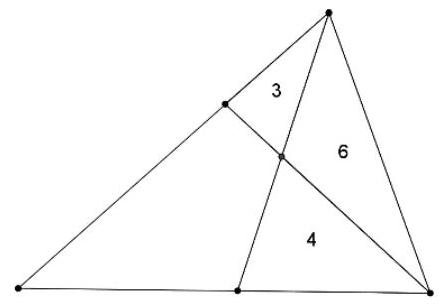
\includegraphics[max width=\textwidth, center]{2024_11_21_ec1df8d0df9314a06be5g-1}
\end{enumerate}

\section*{KLASY TRZECIE}
\begin{enumerate}
  \item Punkt P leży wewnątrz trójkąta \(A B C\). Punkty \(D, E, F\) są punktami symetrycznymi do punktu P odpowiednio względem prostych BC, CA, AB. Wykaż, że jeżeli trójkąt DEF jest równoboczny, to proste \(A D, B E, C F\) przecinają się w jednym punkcie.
  \item Dany jest czworokąt wypukły ABCD. Punkty K i L są odpowiednio środkami boków AB i CD. Wykaż, że jeżeli pola czworokątów BCLK i DAKL są równe, to czworokąt ABCD jest trapezem.
  \item Okrąg K o środku w punkcie I jest styczny do ramion kąta wypukłego XAY w punktach S i\\
T. Udowodnij, że środek okręgu wpisanego w trójkąt SAT leży na okręgu K.
\end{enumerate}

\end{document}